\chapter{Methodology}
\label{chapterlabel5}
In order to identify the uncertainty of modelling assumptions, a patient-specific model of a healthy aorta has been run. In this section, the simulation set up and the choice of the different modelling assumptions is explained.



\section{Patient data}
The patient data was obtained from the Beijing Institute of Technology. The dataset included several aortae from a small patient cohort and flowrate and luminal area waveform at the inlet and the outlets obtained via 4D-Flow MRI and cine-MRI. Additionally, the systolic and diastolic measurements and the heart rate of the patient were included in the measurements as well. \par 

\section{0D model}
The whole system is initially described as a lumped parameter model or also called the 0D model (as explained in Chapter \ref{chapterlabel3}. The model was simulated in the software 20-sim (Controllab Products B.V., Enschede, The Netherlands). \par

The aorta was divided in sections and each section was represented with elementary building blocks consisting of an inertance (L) and a resistance (R). The whole system can be seen on the Figure \ref{fig:0d}. The parameters of each section were obtained from an steady-state CFD simulation, where the inlet flow rate was measured from the 4D-MRI. The parameters were then calculated as:
\begin{align}
    L = \frac{\rho L}{A_{avg}}
\end{align}
\begin{align}
    R = \frac{\Delta P}{Q_{avg}}
\end{align}
where $\rho$ is the density, $L$ is the length of the segment, $A_{avg}$ is the average length of the section, $\Delta P$ is the pressure drop across the section and $Q_{avg}$ is the average flow rate at the section obtained from the patient's MRI dataset.\par

\begin{figure}[ht!]
  \centering
  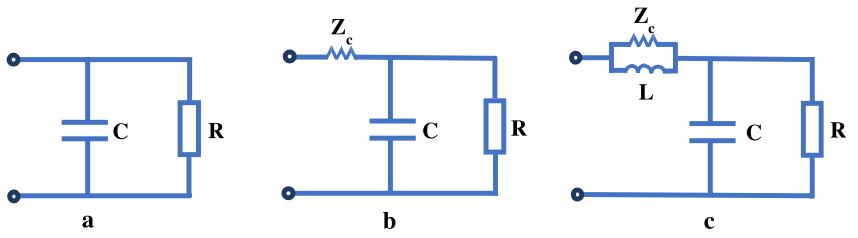
\includegraphics[width=\textwidth]{Figures/WK.JPG}
  \caption{Windkessel models \textbf{a} two-element; \textbf{b} three-element; \textbf{c} four-element \cite{Zhou2019APressure}}
  \label{fig:wind}
\end{figure}

To account for the interaction of the cardiac stroke volume with the compliance of the vessel, an electronic analogous model has been introduced at the outlets, a Windkessel model (different types shown in Figure \ref{fig:wind}). Three-element Windkessel (WK3) model is often used theoretical research. The circuit diagram of the model can be seen on Figure \ref{fig:0d}. \par

\begin{figure}[ht!]
  \centering
  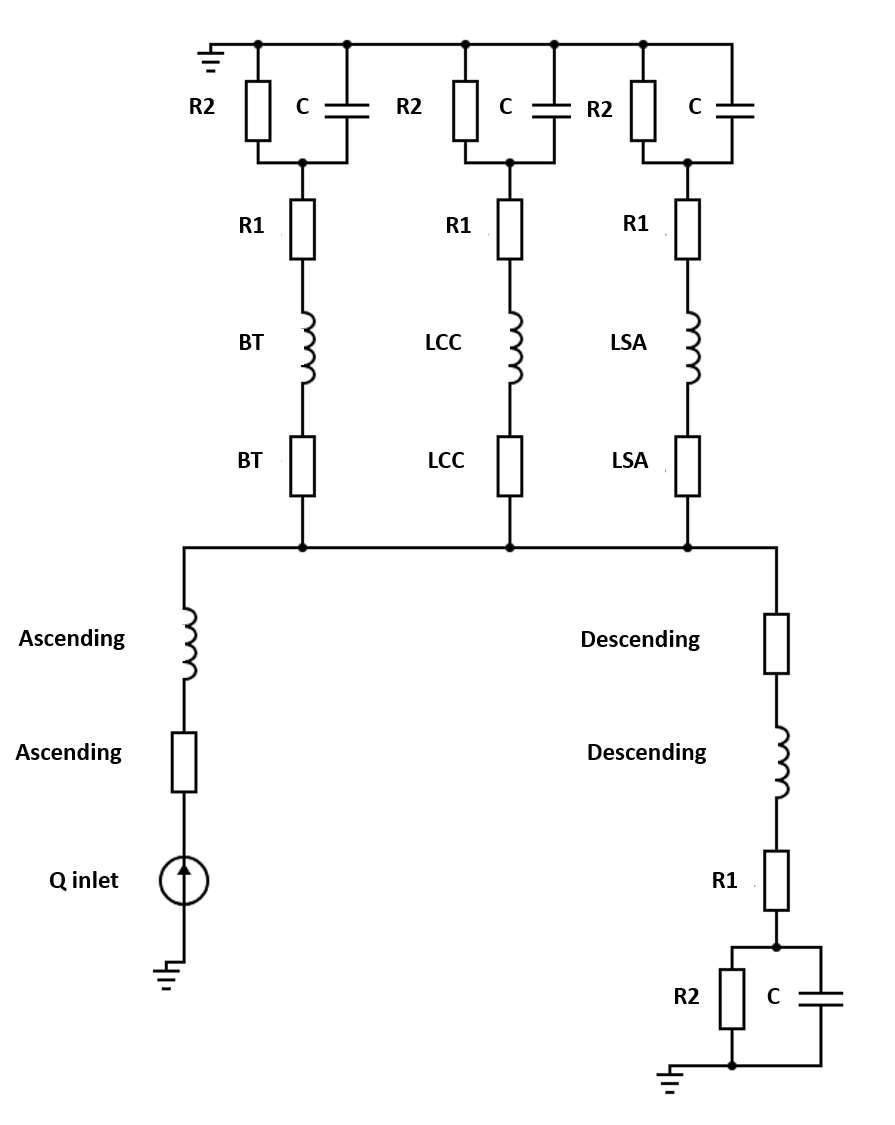
\includegraphics[width=0.5\textwidth]{Figures/circuit.png}
  \caption{Schematic of the 0D model of the aorta}
  \label{fig:0d}
\end{figure}


\subsection{Parameter tuning}
In order to get accurate patient-specific parameters for the given pressure measurements and flow rates, an optimization algorithm was used to tune the individual components of the WK3 at every outlet. \par

Initially, the whole system is described as a single WK3 model where the $R_1$ and $R_2$ have been set as a ratio $R_1/(R_1+R_2) = 5.6\%$ which simplifies the problem to only two parameters $R_1$ and $C$ that need to be fitted. The objective function minimizes the difference between the target systolic and diastolic pressure and the maximum and minimum pressure of the WK3 pressure curve which then gives:
\begin{align}
    min \sqrt{(P_{sys}-P_{max})^2+(P_{dia}-P_{min})^2}
\end{align}
 Additionally, non-negative constraints and bounding constraints have been applied for the parameters between the bounds [0, 2]. \par

Obtaining the parameters for the whole system, the total compliance is distributed proportionally to $\bar{Q_i}$ to the outlets and the resistances are set as a ratio as seen previously. Therefore, for the aorta, at each of the outlet, only one parameter needs to be optimized. The objective function sums up the difference in the target and model pulse pressure, and also the target and the model mean flow rate. As for the whole system model, non-negative constraints and bounding constraints were applied to the parameters. The objective function to be minimized is as following:
\begin{align}
    min \sqrt{(P_{sys}-P_{max})^2+(P_{dia}-P_{min})^2+\sum_{i}(\bar{Q}_{i}^{target}-\bar{Q}_{i}^{0D})^2}
\end{align}
The optimization method used to tune the parameter used was the Broyden–Fletcher–Goldfarb–Shanno algorithm.

\section{Boundary conditions}
The simulations were set up in ANSYS-CFX 19.0 (ANSYS Inc., PA, USA). The blood is modelled as incompressible with a density 1060 $kg m^{-3}$ and the flow was considered laminar, which is a common assumption in large arteries \cite{Alimohammadi2014DevelopmentConditions,Bonfanti2017ComputationalData}. The inlet condition was obtained from 4D-MRI and a flow rate was applied.\par

The three-element Windkessel parameters obtained from the 0D model were coupled to the outlet, relating the mean pressure (P) and the flow (Q) at the outlet via equation \ref{eq:PQ}
\begin{align}
    P=(R_1+R_2)Q-R_2C\frac{dP}{dt}+R_1R_2C\frac{dQ}{dt}
    \label{eq:PQ}
\end{align}
where $R_1$, $R_2$ and $C$ are the parameters obtained for each of the outlet. \par

A no-slip condition was applied, and the wall was considered as rigid. \par

\section{Modelling assumptions}
Different modelling assumptions can be used while modelling a patient aorta. The choice is often justified by the modeler but the resulting simulations can yield significantly different results. In this section, different modelling assumptions that were taken into account are discussed.

\subsection{Segmentation}
While the patient geometries were obtained from the images, the segmentation criterion can affect the resulting geometry primarily affecting the lumen's area. \par

To account for variation in the segmentation, two additional geometries were used, where the patient's aorta was dilated by 0.6 mm creating an expanded and narrow geometry. The amount of variation was based on the voxel size (1 mm) from which the aorta was segmented. \par

\subsection{Image processing}
Depending on the image processing choices and algorithm, smoothing can be applied to the segmentation of the aorta to account for the artefacts in the patient scans. \par

In the simulations two different aortas are being used, where one surface is smooth and the other is unsmooth as seen on the Figure \ref{fig:geometry}.

\begin{figure}[ht!]
    \centering
    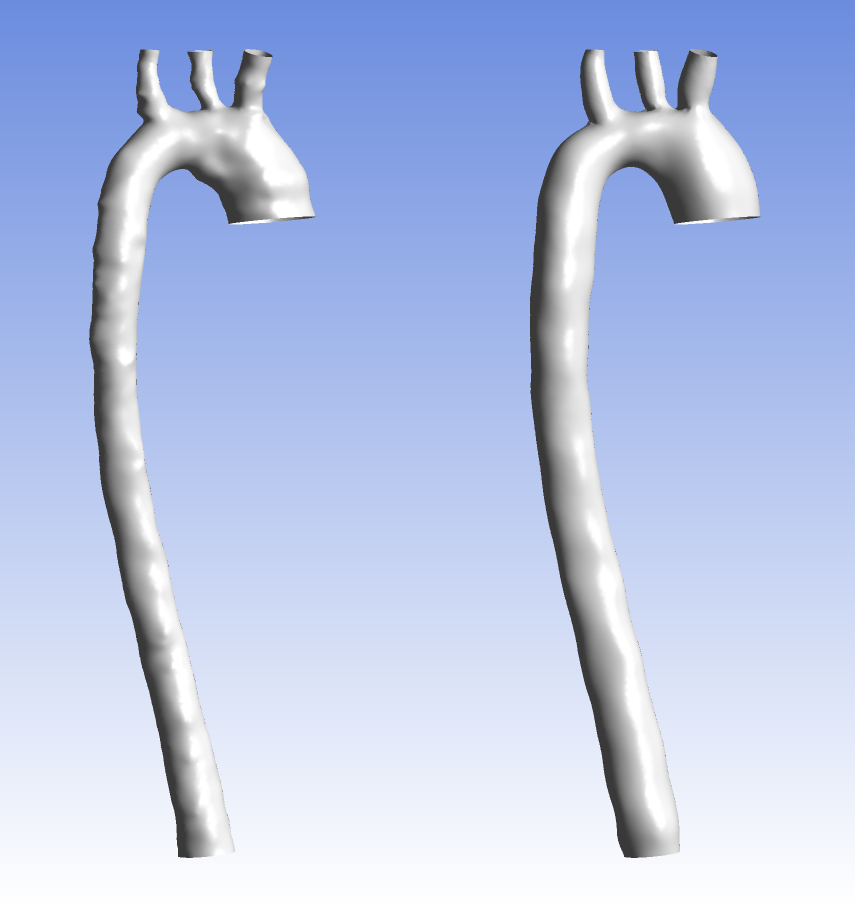
\includegraphics[width=0.5\textwidth]{Figures/Geometry.png}
    \caption{Unsmooth geometry (left) and smooth geometry (right used in the study which can be a result of decisions made during image processing}
    \label{fig:geometry}
\end{figure}

\subsection{Mesh}
While a finer mesh can yield much more accurate results, it comes with a trade-off of computational run time. In CFD simulations, it is  good practice to run mesh sensitivity studies before running the full simulation, however the decision on the mesh quality and approriateness is often left to the modeler.\par

In this project a several meshes were used to  assess how much the mesh can influence the final results. Four different meshes have been used with ~120,000 ~250,000, ~600,000, and ~1,100.000 elements (through this report, the different mesh models will be referred to as Mesh 1-4 models, where Mesh 1 is the coarsest mesh and Mesh 4 is the finest). All meshes were created in ANSYS Fluent (ANSYS Inc., PA, USA). \par

\subsection{Viscosity}
As seen in the Chapter \ref{chapterlabel2}, while blood has shearing properties it is often assumed as Newtonian in larger arteries. Another commonly used approximation, often used in simulations is the Carreau-Yasuda model to model non-Newtonian behaviour. \par

For this work, two blood models have been considered, a Newtonian model with a constant viscosity of 0.004 $Pa$ $s$ and a non-Newtonian model was modelled via the Carreau-Yasuda model, with the parameters taken from the Gijsen et al \cite{Gijsen1999TheModel}.

\section{Conceptual framework to assess structural uncertainty}
The conceptual framework uses permutations of assumptions to build additional models to analyse the uncertainty. By creating additional simulations, the variations across a number of simulation can be assess and the structural uncertainty can be addressed. In addition, study the variability of individual assumptions, it will be possible to evaluate the interacting error due to several assumptions.  \par

By combining the assumptions mentioned above, the framework for a single patient results in 48 different CFD models. \par


\section{Numerical simulations and post-processing}
The simulations run until reaching the periodic steady-state, which was achieved after running three cardiac cycles. For the analysis, the last cycle was used for analysis of the flow and calculation of the time-averaged wall shear stress (TAWSS). 

\begin{equation}
TAWSS=\frac{1}{T}\int_{0}^{T} |\tau(t)|dt
\label{eq:tawss}
\end{equation}
where $|\tau(t)|$ is the magnitude of WSS at the time $t$. \par

The post-processing was done in CFD-Post (ANSYS Inc., PA, USA) and by Python (Python Software Foundation, DE, USA).

